\documentclass{SelimArticle}
\definecolor{RosyBrown}{rgb}{0.737255,0.560784,0.560784}
\definecolor{light goldenrod}{rgb}{0.933333,0.866667,0.509804}
\definecolor{LightGoldenrod}{rgb}{0.933333,0.866667,0.509804}
\definecolor{Sienna}{rgb}{0.627451,0.321569,0.176471}
\definecolor{Red}{rgb}{0.803922,0.000000,0.000000} %Actually red3
%\definecolor{Red}{rgb}{0.803922,0.360784,0.360784} %Actually Indian Red
%\definecolor{Red}{rgb}{0.815686,0.125490,0.564706} %Actually Violet Red
%\definecolor{Red}{rgb}{1.000000,0.270588,0.000000} %Actually Orange Red
%\definecolor{Red}{rgb}{0.545098,0.227451,0.227451} %Actually Indian Red 4
\sectionfont{ \sectionrule{0pt}{0pt}{-5pt}{0.8pt} }  %Horizontal line below section.
\setcounter{secnumdepth}{2}  % Numbering of sections and subsections
\usepackage{amsmath}
\usepackage{pdfpages}
\usepackage[refpage]{nomencl}
\usepackage{multirow}
\usepackage{bigstrut}
\usepackage{pdfpages}
\usepackage{setspace} %allows double spacing with \doublespacing command
\usepackage{pdflscape}
\usepackage[graphicx]{realboxes}
\setlength{\nomitemsep}{-\parsep}
\usepackage[linktoc=all]{hyperref} %allows me to make a hyperref table of contents
\hypersetup{
    colorlinks,
    citecolor=black,
    filecolor=black,
    linkcolor=black,
    urlcolor=black
}

%Used for nomenclature making
\renewcommand*{\pagedeclaration}[1]{\unskip\dotfill\hyperpage{#1}}
\makenomenclature
%In CMD, makeindex <filename>.nlo -s nomencl.ist -o <filename>.nls

%%%%%%%%%%%%%%%%%%%%
%EDIT TITLE PAGE%%%%
%\course{Mechanics of Composite Materials}        
%\coursenum{MECH-530} 
%\title{Project - Part 1 \\ Python Code Output}   %Add \\[0.3cm] for other line. 
%\student{Elaine \textsc{Craigie}}  %Simple \\ to add more names. Don't forget \textsc
%\studentnum{260476434}
%\vspace{3cm}
%\date{\today}
%EDIT TITLE PAGE%%%%%
%%%%%%%%%%%%%%%%%%%%%
%%%%%%%%%%%%%%%%%%%%%%%%%%%%%%%%%%%%%%%%%
% Classic Lined Title Page 
% LaTeX Template
% Version 1.0 (27/12/12)
%
% This template has been downloaded from:
% http://www.LaTeXTemplates.com
%
% Original author:
% Peter Wilson (herries.press@earthlink.net)
%
% License:
% CC BY-NC-SA 3.0 (http://creativecommons.org/licenses/by-nc-sa/3.0/)
% 
% Instructions for using this template:
% This title page compiles as is. If you wish to include this title page in 
% another document, you will need to copy everything before 
% \begin{document} into the preamble of your document. The title page is
% then included using \titleAT within your document.
%
%%%%%%%%%%%%%%%%%%%%%%%%%%%%%%%%%%%%%%%%%

%----------------------------------------------------------------------------------------
%	PACKAGES AND OTHER DOCUMENT CONFIGURATIONS
%----------------------------------------------------------------------------------------

\newcommand*{\plogo}{\fbox{$\mathcal{PL}$}} % Generic publisher logo

%----------------------------------------------------------------------------------------
%	TITLE PAGE
%----------------------------------------------------------------------------------------

\newcommand*{\titleAT}{\begingroup % Create the command for including the title page in the document
\newlength{\drop} % Command for generating a specific amount of whitespace
\drop=0.1\textheight % Define the command as 10% of the total text height

\rule{\textwidth}{1pt}\par % Thick horizontal line
\vspace{2pt}\vspace{-\baselineskip} % Whitespace between lines
\rule{\textwidth}{0.4pt}\par % Thin horizontal line

\vspace{\drop} % Whitespace between the top lines and title
\centering % Center all text
\textcolor{Red}{ % Red font color
{\Huge TERM PROJECT}\\[0.5\baselineskip] % Title line 1
{\Large MECH-530}\\[0.75\baselineskip] % Title line 2
{\Huge Progress Report 5}} % Title line 3

\vspace{0.25\drop} % Whitespace between the title and short horizontal line
\rule{0.3\textwidth}{0.4pt}\par % Short horizontal line under the title
\vspace{\drop} % Whitespace between the thin horizontal line and the author name

{\Large \textsc{Elaine Craigie} \\ \vspace{0.5cm} (260476434)}\par % Author name

\vfill % Whitespace between the author name and publisher text
%{\large \textcolor{Red}{\plogo}}\\[0.5\baselineskip] % Publisher logo

\includegraphics[scale = 0.45]{pic_mcgill}
\vspace{2.0cm}
{\Large \\ \today}\par % Publisher
\vspace{1.0cm}
{\raggedleft{}
\textcolor{Red}{
{\large \\ \textsc{Overview:} This progress report features the addition of a module to analyze various failure criterion, notably Maximum Stress, Quadratic Polynomial and Hashin Criterion. The purpose of this analysis is to determine how close the laminate is to failure as well as the mode of the eventual failure, where applicable.}}}
\centering
\rule{\textwidth}{0.4pt}\par % Thin horizontal line
\vspace{2pt}\vspace{-\baselineskip} % Whitespace between lines
\rule{\textwidth}{1pt}\par % Thick horizontal line

\endgroup}

%----------------------------------------------------------------------------------------
%	BLANK DOCUMENT
%----------------------------------------------------------------------------------------
\begin{document}
\pagestyle{empty} % Removes page numbers

\titleAT % This command includes the title page
%%%%%%%%%%%%%%%%%%%%

%\mytitlepage
%\pagenumbering{roman}
%\setcounter{page}{1}
%\doublespacing
%\tableofcontents
%\newpage
%\renewcommand{\nomname}{List of Symbols}
\printnomenclature[0.5in]
\newpage
\pagenumbering{arabic}
\setcounter{page}{1}
\section{Preliminary Calculations and Design Criterion}
Based on the following given parameters, the applied load vectors were obtained. Thus, $M_{1} =$ -1159.09~N while $M_{2} = M_{6} = 0$~N, and $N_{1} =$ 4545.45~N/m (tensile load) while $N_{2} = N_{6} = 0$~N/m.

\begin{itemize}
\item L = 51 cm (length of skateboard)
\item b = 11 cm (width of skateboard)
\item $P_{1}$ = 1000~N downwards (arbitrary load) 
\end{itemize}
 
\begin{align*}
M_{1} &= \frac{M}{b} \\
&= \frac{P_{1} \cdot L}{4 \cdot b} \\
&= \frac{-1000 \cdot 0.51}{4 \cdot 0.11} \\
&= -1159.0909~\text{N}
\end{align*}

\begin{align*} 
N_{1} &= \frac{0.5 \cdot |P_{1}|}{b} \\
&= \frac{1000}{2 \cdot 0.11} \\
&= 4545.4545~\text{N/m}
\end{align*}

Refer to the tables in Sections~\ref{tab:stress_strain}~and~\ref{tab:failure}~for the stresses, strains and failure $R$ values per top and bottom of each ply.

\section{Program Output}
\label{sec:programout}
Program output to follow...
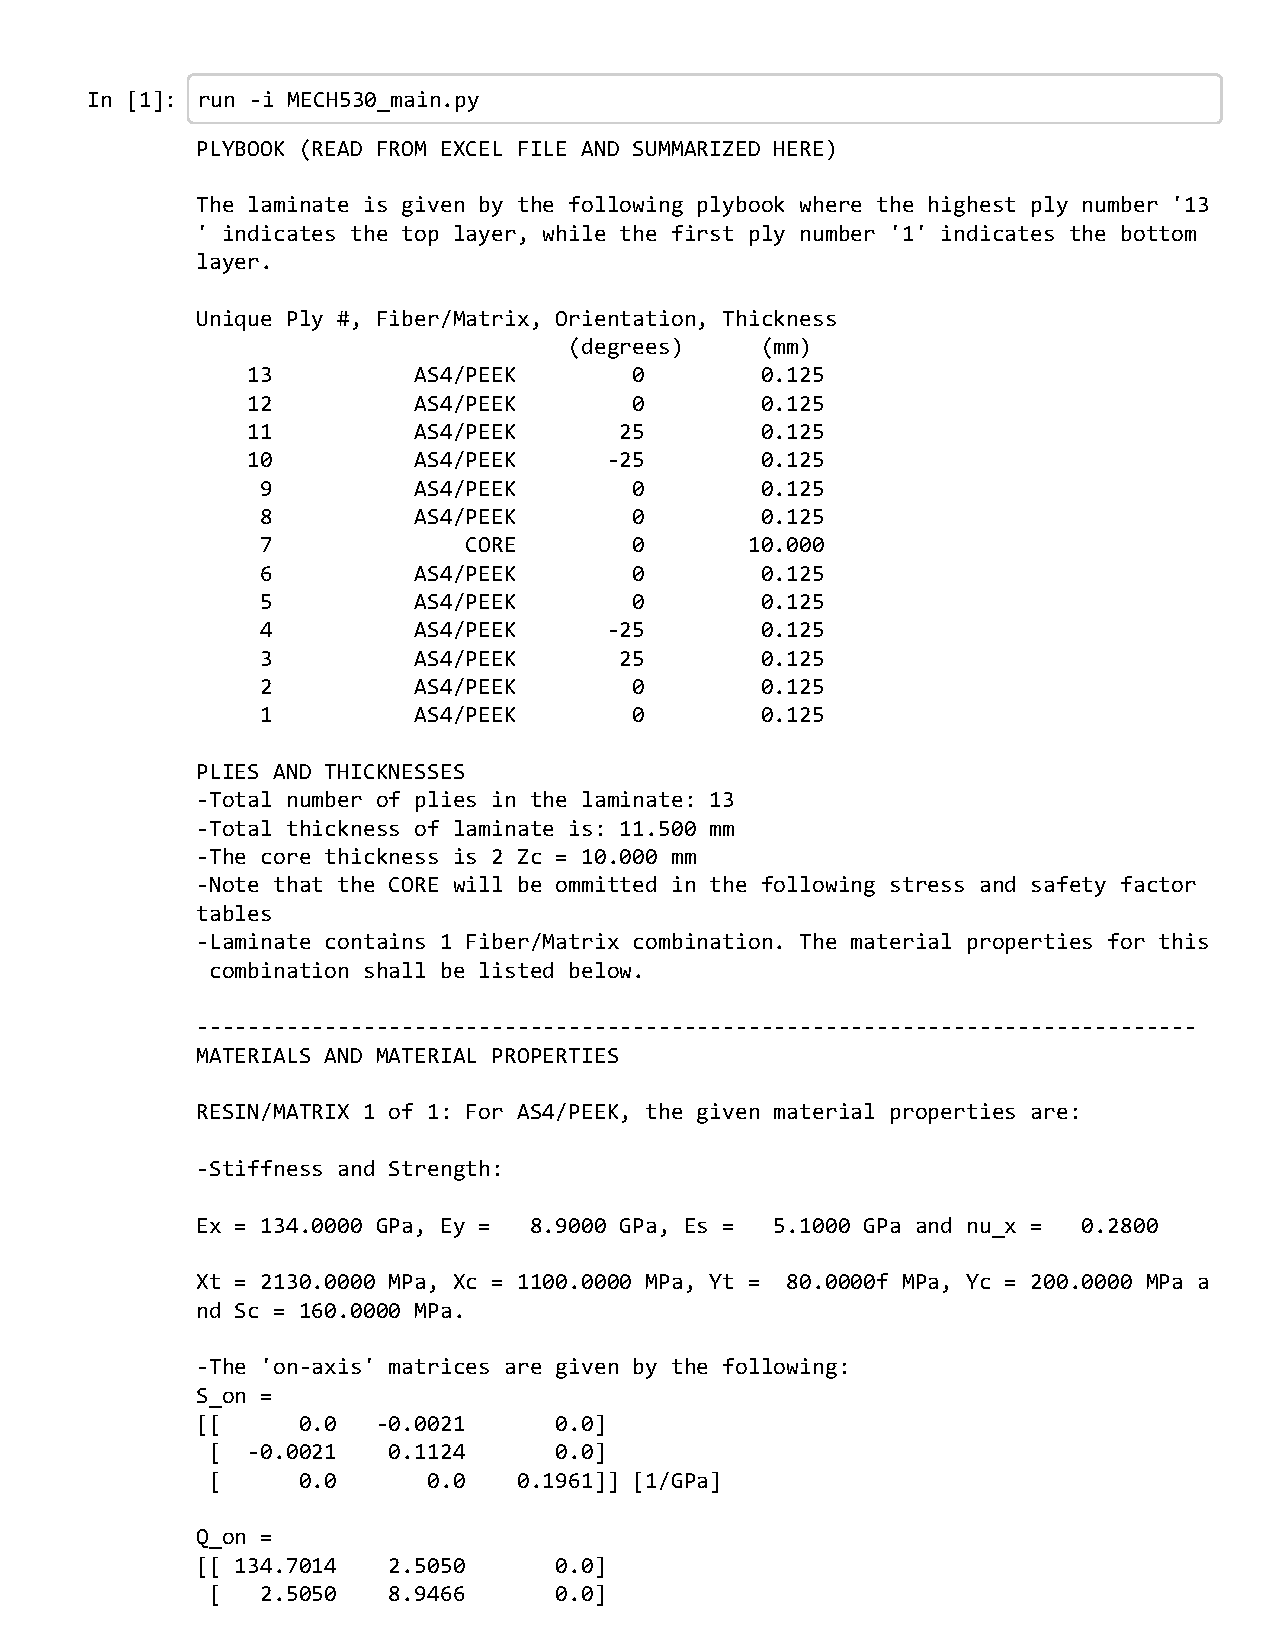
\includepdf[pages={1-3}]{MECH530_Ass5_notebook.pdf}

\appendix
\section{Stress and Strain State throughout Laminate}
\label{tab:stress_strain}
\Rotatebox{90}{%
\centering
\begin{tabular}{cccccccccccc}
\toprule
Position &  Ply &  Angle & $\epsilon_{1}$ & $\epsilon_{2}$ & $\epsilon_{6}$ & $\epsilon_{x}$ & $\epsilon_{y}$ & $\epsilon_{s}$ & $\sigma_{x}$ & $\sigma_{y}$ & $\sigma_{s}$ \\
\midrule
 & & ($^{o}$) & & & & & & & (GPa) & (GPa) & (GPa) \\
TOP &   13 &            0 & -0.001309 &  0.001017 &  0.000030 & -0.001309 &  0.001017 &  0.000030 &      -0.173735 &       0.005822 &       0.000151 \\
BOT &   13 &            0 & -0.001280 &  0.000995 &  0.000029 & -0.001280 &  0.000995 &  0.000029 &      -0.169882 &       0.005693 &       0.000148 \\
TOP &   12 &            0 & -0.001280 &  0.000995 &  0.000029 & -0.001280 &  0.000995 &  0.000029 &      -0.169882 &       0.005693 &       0.000148 \\
BOT &   12 &            0 & -0.001251 &  0.000972 &  0.000028 & -0.001251 &  0.000972 &  0.000028 &      -0.166029 &       0.005564 &       0.000145 \\
TOP &   11 &           25 & -0.001251 &  0.000972 &  0.000028 & -0.000843 &  0.000564 &  0.001721 &      -0.112111 &       0.002937 &       0.008777 \\
BOT &   11 &           25 & -0.001222 &  0.000950 &  0.000028 & -0.000823 &  0.000551 &  0.001681 &      -0.109508 &       0.002868 &       0.008573 \\
TOP &   10 &          -25 & -0.001222 &  0.000950 &  0.000028 & -0.000844 &  0.000572 & -0.001645 &      -0.112318 &       0.003005 &      -0.008391 \\
BOT &   10 &          -25 & -0.001193 &  0.000927 &  0.000027 & -0.000824 &  0.000559 & -0.001606 &      -0.109650 &       0.002934 &      -0.008192 \\
TOP &    9 &            0 & -0.001193 &  0.000927 &  0.000027 & -0.001193 &  0.000927 &  0.000027 &      -0.158323 &       0.005306 &       0.000138 \\
BOT &    9 &            0 & -0.001164 &  0.000904 &  0.000026 & -0.001164 &  0.000904 &  0.000026 &      -0.154470 &       0.005177 &       0.000135 \\
TOP &    8 &            0 & -0.001164 &  0.000904 &  0.000026 & -0.001164 &  0.000904 &  0.000026 &      -0.154470 &       0.005177 &       0.000135 \\
BOT &    8 &            0 & -0.001135 &  0.000882 &  0.000026 & -0.001135 &  0.000882 &  0.000026 &      -0.150618 &       0.005047 &       0.000132 \\
TOP &    6 &            0 &  0.001187 & -0.000923 & -0.000026 &  0.001187 & -0.000923 & -0.000026 &       0.157615 &      -0.005282 &      -0.000132 \\
BOT &    6 &            0 &  0.001216 & -0.000945 & -0.000026 &  0.001216 & -0.000945 & -0.000026 &       0.161468 &      -0.005411 &      -0.000135 \\
TOP &    5 &            0 &  0.001216 & -0.000945 & -0.000026 &  0.001216 & -0.000945 & -0.000026 &       0.161468 &      -0.005411 &      -0.000135 \\
BOT &    5 &            0 &  0.001245 & -0.000968 & -0.000027 &  0.001245 & -0.000968 & -0.000027 &       0.165320 &      -0.005540 &      -0.000138 \\
TOP &    4 &          -25 &  0.001245 & -0.000968 & -0.000027 &  0.000860 & -0.000583 &  0.001678 &       0.114435 &      -0.003061 &       0.008558 \\
BOT &    4 &          -25 &  0.001274 & -0.000991 & -0.000028 &  0.000880 & -0.000597 &  0.001717 &       0.117102 &      -0.003132 &       0.008757 \\
TOP &    3 &           25 &  0.001274 & -0.000991 & -0.000028 &  0.000859 & -0.000575 & -0.001753 &       0.114293 &      -0.002995 &      -0.008939 \\
BOT &    3 &           25 &  0.001303 & -0.001013 & -0.000028 &  0.000879 & -0.000588 & -0.001793 &       0.116895 &      -0.003064 &      -0.009143 \\
TOP &    2 &            0 &  0.001303 & -0.001013 & -0.000028 &  0.001303 & -0.001013 & -0.000028 &       0.173026 &      -0.005799 &      -0.000145 \\
BOT &    2 &            0 &  0.001332 & -0.001036 & -0.000029 &  0.001332 & -0.001036 & -0.000029 &       0.176879 &      -0.005928 &      -0.000148 \\
TOP &    1 &            0 &  0.001332 & -0.001036 & -0.000029 &  0.001332 & -0.001036 & -0.000029 &       0.176879 &      -0.005928 &      -0.000148 \\
BOT &    1 &            0 &  0.001361 & -0.001058 & -0.000030 &  0.001361 & -0.001058 & -0.000030 &       0.180732 &      -0.006057 &      -0.000151 \\
\bottomrule
\end{tabular}
}%

\section{Failure Criterion R Values}
\label{tab:failure}

\Rotatebox{90}{%
\centering
\begin{tabular}{cccccccccccccc}
\toprule
 & & & \multicolumn{5}{|c}{Maximum Stress} & \multicolumn{2}{|c}{Quad Poly} & \multicolumn{4}{|c}{Hashin Criterion} \\
\midrule
Position & Ply & Angle & FT & FC & MT & MC & S & (+) & (-) & FT & FC & MT & MC \\
\midrule
 & & ($^{o}$) & & & & & & & & & & & \\
TOP      & 13 &        0 &  0.000 &  6.331 & 13.741 &  0.000 & 1057.104 &  4.664 & -10.599 &  0.000 &  6.331 & 13.740 &  0.000 \\
BOT      & 13 &        0 &  0.000 &  6.475 & 14.052 &  0.000 & 1080.595 &  4.770 & -10.840 &  0.000 &  6.475 & 14.051 &  0.000 \\
TOP      & 12 &        0 &  0.000 &  6.475 & 14.052 &  0.000 & 1080.595 &  4.770 & -10.840 &  0.000 &  6.475 & 14.051 &  0.000 \\
BOT      & 12 &        0 &  0.000 &  6.625 & 14.378 &  0.000 & 1105.154 &  4.881 & -11.091 &  0.000 &  6.625 & 14.377 &  0.000 \\
TOP      & 11 &       25 &  0.000 &  9.812 & 27.243 &  0.000 &   18.230 &  6.912 & -13.631 &  0.000 &  9.812 & 15.151 &  0.000 \\
BOT      & 11 &       25 &  0.000 & 10.045 & 27.890 &  0.000 &   18.663 &  7.077 & -13.955 &  0.000 & 10.045 & 15.511 &  0.000 \\
TOP      & 10 &      -25 &  0.000 &  9.794 & 26.620 &  0.000 &   19.067 &  6.931 & -13.817 &  0.000 &  9.794 & 15.501 &  0.000 \\
BOT      & 10 &      -25 &  0.000 & 10.032 & 27.267 &  0.000 &   19.531 &  7.099 & -14.153 &  0.000 & 10.032 & 15.878 &  0.000 \\
TOP      &  9 &        0 &  0.000 &  6.948 & 15.078 &  0.000 & 1157.780 &  5.119 & -11.631 &  0.000 &  6.948 & 15.077 &  0.000 \\
BOT      &  9 &        0 &  0.000 &  7.121 & 15.454 &  0.000 & 1186.019 &  5.246 & -11.921 &  0.000 &  7.121 & 15.453 &  0.000 \\
TOP      &  8 &        0 &  0.000 &  7.121 & 15.454 &  0.000 & 1186.019 &  5.246 & -11.921 &  0.000 &  7.121 & 15.453 &  0.000 \\
BOT      &  8 &        0 &  0.000 &  7.303 & 15.850 &  0.000 & 1215.669 &  5.380 & -12.226 &  0.000 &  7.303 & 15.848 &  0.000 \\
TOP      &  6 &        0 & 13.514 &  0.000 &  0.000 & 37.863 & 1215.669 & 11.683 &  -5.141 & 13.513 &  0.000 &  0.000 & 37.836 \\
BOT      &  6 &        0 & 13.192 &  0.000 &  0.000 & 36.959 & 1186.019 & 11.405 &  -5.019 & 13.191 &  0.000 &  0.000 & 36.934 \\
TOP      &  5 &        0 & 13.192 &  0.000 &  0.000 & 36.959 & 1186.019 & 11.405 &  -5.019 & 13.191 &  0.000 &  0.000 & 36.934 \\
BOT      &  5 &        0 & 12.884 &  0.000 &  0.000 & 36.098 & 1157.780 & 11.139 &  -4.902 & 12.883 &  0.000 &  0.000 & 36.073 \\
TOP      &  4 &      -25 & 18.613 &  0.000 &  0.000 & 65.339 &   18.696 & 13.557 &  -6.802 & 13.191 &  0.000 &  0.000 & 16.892 \\
BOT      &  4 &      -25 & 18.189 &  0.000 &  0.000 & 63.851 &   18.270 & 13.248 &  -6.647 & 12.890 &  0.000 &  0.000 & 16.507 \\
TOP      &  3 &       25 & 18.636 &  0.000 &  0.000 & 66.769 &   17.898 & 13.375 &  -6.781 & 12.909 &  0.000 &  0.000 & 16.288 \\
BOT      &  3 &       25 & 18.221 &  0.000 &  0.000 & 65.283 &   17.500 & 13.078 &  -6.630 & 12.622 &  0.000 &  0.000 & 15.925 \\
TOP      &  2 &        0 & 12.310 &  0.000 &  0.000 & 34.490 & 1105.154 & 10.643 &  -4.684 & 12.310 &  0.000 &  0.000 & 34.466 \\
BOT      &  2 &        0 & 12.042 &  0.000 &  0.000 & 33.739 & 1080.595 & 10.411 &  -4.581 & 12.041 &  0.000 &  0.000 & 33.716 \\
TOP      &  1 &        0 & 12.042 &  0.000 &  0.000 & 33.739 & 1080.595 & 10.411 &  -4.581 & 12.041 &  0.000 &  0.000 & 33.716 \\
BOT      &  1 &        0 & 11.785 &  0.000 &  0.000 & 33.020 & 1057.104 & 10.189 &  -4.484 & 11.785 &  0.000 &  0.000 & 32.997 \\
\bottomrule
\end{tabular}
}%

\end{document}